\documentclass[a4paper, 10pt]{article}

\usepackage[utf8]{inputenc}
\usepackage[french]{babel}
\usepackage[T1]{fontenc}
\usepackage{fancyhdr}
\usepackage{amsmath}
\usepackage{framed}
\usepackage[a4paper, margin=2cm]{geometry}
\usepackage{varwidth}
\usepackage[babel=true]{csquotes}
\usepackage{array}
\usepackage{subfig}
\usepackage{pgfplots} %for functions, graphs, etc.
\usepackage{wrapfig}
\usepackage{listings}
\usepackage{subfig}
\usepackage{hyperref}
\usepackage{multicol}


\usepackage{amsfonts}

\usepackage{hyperref}
\expandafter\def\expandafter\UrlBreaks\expandafter{\UrlBreaks%  save the current one
  \do\a\do\b\do\c\do\d\do\e\do\f\do\g\do\h\do\i\do\j%
  \do\k\do\l\do\m\do\n\do\o\do\p\do\q\do\r\do\s\do\t%
  \do\u\do\v\do\w\do\x\do\y\do\z\do\A\do\B\do\C\do\D%
  \do\E\do\F\do\G\do\H\do\I\do\J\do\K\do\L\do\M\do\N%
  \do\O\do\P\do\Q\do\R\do\S\do\T\do\U\do\V\do\W\do\X%
  \do\Y\do\Z}
  
  \lstdefinestyle{customc}{
  belowcaptionskip=1\baselineskip,
  breaklines=true,
  frame=l,
  xleftmargin=\parindent,
  language=C++,
  showstringspaces=false,
  basicstyle=\footnotesize\ttfamily,
  keywordstyle=\bfseries\color{green!40!black},
  commentstyle=\itshape\color{purple!40!black},
  identifierstyle=\color{blue},
  stringstyle=\color{purple},
}
  
  \lstset{
basicstyle=\footnotesize\ttfamily,
style=customc,
inputencoding=latin1,
language={C++},
breaklines=true,
showstringspaces=false,
literate=%
		 {á}{{\'a}}1 {à}{{\`a}}1 {í}{{\'i}}1 {é}{{\'e}}1 {è}{{\`e}}1 {ý}{{\'y}}1
		 {ú}{{\'u}}1 {ó}{{\'o}}1 {ô}{{\^o}}1 {ě}{{\v{e}}}1 {š}{{\v{s}}}1 {č}{{\v{c}}}1
		 {ř}{{\v{r}}}1 {ž}{{\v{z}}}1 {ď}{{\v{d}}}1 {ť}{{\v{t}}}1 {ň}{{\v{n}}}1
		 {ů}{{\r{u}}}1 {Á}{{\'A}}1 {Í}{{\'I}}1 {É}{{\'E}}1 {Ý}{{\'Y}}1 {Ú}{{\'U}}1
		 {Ó}{{\'O}}1 {Ě}{{\v{E}}}1 {Š}{{\v{S}}}1 {Č}{{\v{C}}}1 {Ř}{{\v{R}}}1 {Ž}{{\v{Z}}}1
		 {Ď}{{\v{D}}}1 {Ť}{{\v{T}}}1 {Ň}{{\v{N}}}1                {Ů}{{\r{U}}}1
}

\author{Antonin Godard (2032402), Rayan Neggazi (2038882)}
\title{\sffamily\textbf{[INF8500] Rapport lab 2}}

\lstset{numbers=left, numberstyle=\tiny, numbersep=5pt}

\begin{document}

\maketitle

\begin{figure}[htb]
	\centering
	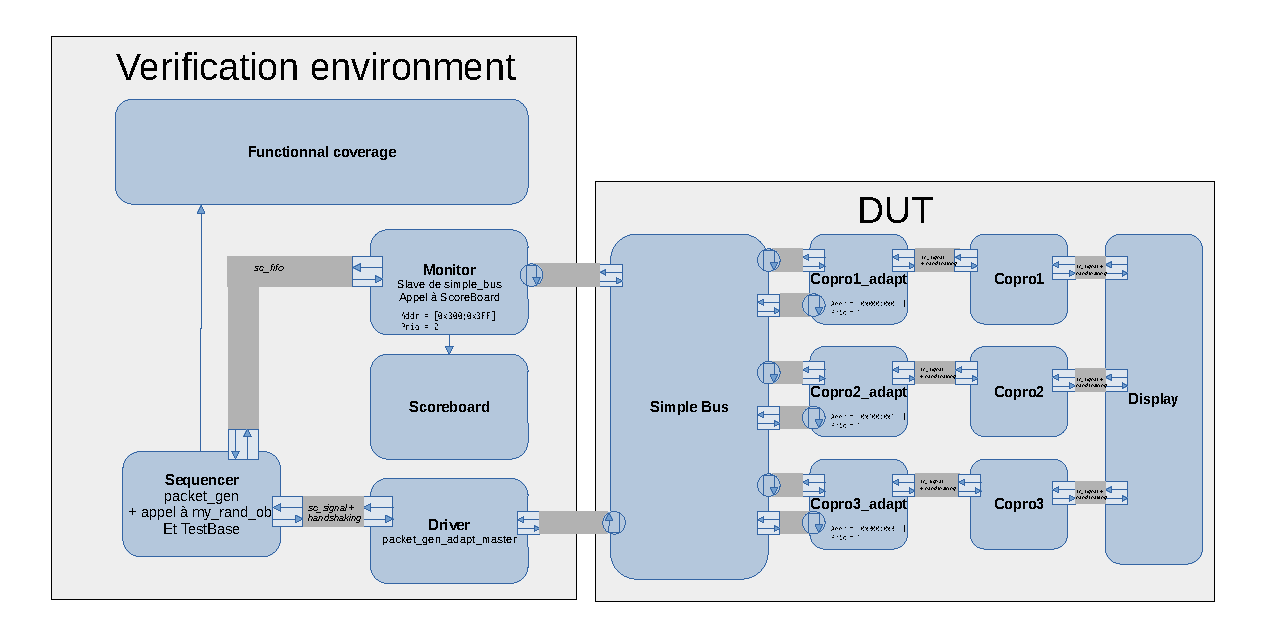
\includegraphics[width=\linewidth]{schema.pdf}
	\caption{Schema}
	\label{fig:schema}
\end{figure}

\begin{enumerate}
	\item Le schéma figure~\ref{fig:schema} page~\pageref{fig:schema} représente notre
		système final (zoom possible pour les détails). On détaille chaque bloc :
		\begin{itemize}
			\item \textbf{Functionnal coverage} est le bloc qui fait la vérification fonctionnelle
				du système et représente la classe TestBase. On utilise la bibliothèque FC4SC.
				
				Cette classe est instanciée dans \texttt{packet\_gen} et on sample chaque
				paramètre de notre système (les copros, les différents tris et la
				direction du tri) directement à chaque tour de boucle.

				Nos résultats se trouvent à la figure~\ref{fig:fc4sc}
				page~\pageref{fig:fc4sc}. Le fichier xml est également présent à la source
				de notre rendu.

			\item \textbf{Sequencer} est le bloc représentant \texttt{packet\_gen}. Ce bloc génère
				les paquets qui vont être envoyés aux coprocesseurs.

				Il procède en cinq phases :
				\begin{enumerate}
					\item Génération d'une nouvelle addresse, d'un type de données et d'une
						direction de tri avec \texttt{my\_rand\_obj}.
					\item Sample des valeurs générées par \texttt{my\_rand\_obj} pour la
						couverture fonctionnelle.
					\item Génération des données destinées à être triée avec \texttt{TestBase} en fonction
						du type de données généré par \texttt{my\_rand\_obj}.
					\item Envoi du paquet au moniteur via \emph{un canal FIFO}, avec l'appel
						\texttt{nb\_write} pour ne pas bloquer le générateur.\footnote{En
						fait dans notre modèle si on faisait simplement un \texttt{write}
						le système bloquerait car le moniteur n'effectue un \texttt{read}
						sur la FIFO seulement lorsqu'il reçoit un paquet des copros}
					\item Création du nouveau  paquet avec les données générées précedemment ainsi
						que l'addresse de \texttt{my\_rand\_obj}, puis envoi au Driver via un
						canal \texttt{sc\_signal} et un handshaking.
				\end{enumerate}

				\item Le \textbf{Driver} reçoit les données du générateur (Sequencer)
					puis les envoient à la bonne addresse via le Simple Bus. Il fait un
					appel bloquant \texttt{burst\_write}.

				\item Chaque \textbf{Copro*\_Adapt} agit ici comme un esclave et comme
					un maître. C'est un esclave car il reçoit les paquets du Driver,
					comme au lab 1. C'est également un maître car il envoie les
					données triées au Moniteur avec un appel bloquant
					\texttt{burst\_write}.
					
					Il envoie également les données triées au display via un
					\texttt{sc\_signal} et un handshaking.

					Il sont définis sur les plages \texttt{[0x000; 0x0FF]},
					\texttt{[0x100; 0x1FF]}, et \texttt{[0x200; 0x3FF]}, et ont chacun une
					priorité de 1, supérieure au moniteur.

				\item Le \textbf{Moniteur} est un esclave qui reçoit un paquet de la
					part du Séquenceur ainsi que des coprocesseurs. Il a pour rôle de
					comparer les deux paquets en instanciant la classe
					\texttt{ScoreBoard} et en appelant la méthode \texttt{check\_int}
					de cette dernière.

					Il est de priorité inférieure aux adaptateurs de coprocesseurs (=2) et
					est défini sur la plage d'addresse \texttt{[0x300; 0x3FF]}.

				\item Le \textbf{ScoreBoard} compare les pointeurs de chaque paquets.
					Sa fonctionnalité pourrait être améliorée en comparant réellement
					les deux contenus de chaque payload de paquets, en triant le
					contenu du paquet en provenance du Séquenceur au préalable en
					utilisant une fonction de tri fiable.
		\end{itemize}

	\item Nous avons réalisé notre couverture fonctionnelle à l’aide de la librairie
		FC4SC.  Pour le groupe de couverture nous avons créé la classe \texttt{input\_cvg}
		comprenant les variables à couvrir : \texttt{copro}, \texttt{data\_order} et
		\texttt{sort\_dir}.

		\begin{lstlisting}[numbers=none]
class input_cvg : public covergroup
{

public:
  int copro;
  int data_order;
  int sort_dir;
  int nb_de_cov = 0;
		\end{lstlisting}

		Le sampling est alors effectué sur l’ensemble de ces variables, on mesure le
		nombre de 
		couvertures grâce à la variable \texttt{nb\_de\_cov} qui s’incrémente à chaque
		appel de « \texttt{sample} ».

\begin{lstlisting}[numbers=none]
void sample(int copro, int data_order, int sort_dir)
{
	this->copro = copro;
	this->data_order = data_order;
	this->sort_dir = sort_dir;
	covergroup::sample();
	nb_de_cov += 1;
}
\end{lstlisting}

		On crée ensuite une sonde pour chaque variable grâce au macro \texttt{COVERPOINT}. Pour
		chacune des sondes on crée une boîte par valeur que peut prendre la variable,
		ainsi nous pourrons observer les occurrences de chaque valeur une par une et avoir
		une couverture complète.

\begin{multicols}{2}
\begin{lstlisting}[numbers=none]
COVERPOINT(int, copro_cvp, copro){
	bin<int>("copro 1", 0),
	bin<int>("copro 2", 1),
	bin<int>("copro 3", 2),
};
\end{lstlisting}
\begin{lstlisting}[numbers=none]
COVERPOINT(int, sort_dir_cvp, sort_dir){
	bin<int>("up", 1),
	bin<int>("down", 0)};
\end{lstlisting}	
\begin{lstlisting}[numbers=none]
COVERPOINT(int, data_order_cvp, data_order){
	bin<int>("random_desc", 0),
	bin<int>("random_asc", 1),
	bin<int>("random_full", 2),
	bin<int>("continues_asc", 3),
	bin<int>("continues_desc", 4),
};
\end{lstlisting}
\end{multicols}

		Afin de couvrir l’ensemble des combinaisons possibles entre nos variables, nous
		ferons des mesures croisées.

\begin{lstlisting}[numbers=none]
cross<int, int, int> reset_valid_cross = cross<int, int, int>(this,
		"Croisement des 3 parametres",
		&copro_cvp,
		&data_order_cvp,
		&sort_dir_cvp);
\end{lstlisting}

		Les résultats de la simulation sont présentés dans le tableau joint
		figure~\ref{fig:fc4sc} page~\pageref{fig:fc4sc}, nous avons obtenu 100\% ce qui
		signifie que notre couverture a parcouru chacune des combinaisons possibles entre
		les trois variables.

	\item Voici les améliorations que nous avons / aurions pu apporter :
		\begin{itemize}
			\item Un canal FIFO entre le Séquenceur et le Moniteur. Comme mentionné
				précedemment, nous effectuons un \texttt{nb\_write} depuis le Séquenceur,
				ce qui évite de bloquer le Séquenceur (\texttt{packet\_gen}).
				Cependant, nous aurions également pu définir \emph{une taille} à la FIFO
				et également bloquer le Séquenceur lorsque celle-ci est pleine. En faisait
				par exemple :

				\begin{center}
					\verb|if (packet_monitor.num_free() > 0) packet_monitor.nb_write();|
				\end{center}

			\item Le Scoreboard aurait pu être amélioré en implantant une fonction de tri à
				bulles préfaite (ou bien une fonction de tri classique, éventuellement
				plus performante pour accélerer la simulation) et en triant les données
				reçues du Séquenceur. Une fois ces données triées nous les comparons avec
				les données reçues par les coprocesseurs afin de vérifier le bon
				fonctionnement du tri.

			\item Nous avons essayé d'implanter une amélioration pour les tri Ascendant
				Random et Descendant Random. 

				Malheureusement nous obtenions une erreur que nous ne comprenons pas.
				Voici ce que ça aurait donné sinon :

\begin{lstlisting}
struct item_Asc : public crv_sequence_item {
  crv_variable<unsigned> x;

  crv_constraint constr{ x() > x(prev), x() <= x(prev) * 2 };

  item_Asc(crv_object_name) {}
};

int * Test_Random_Asc_data_gen::runphase(int a){

  item_Asc obj("obj");
  static unsigned int n = 0;
  
  for(int i = 0;i<MAX;i++)
  {
    CHECK(obj.randomize());
    n += obj.x;
    iarray[i] = n;
  }
  return iarray;
}

\end{lstlisting}
			
			L'idée est de générer un nouveau \texttt{x} en fonction de sa valeur
			précédente. \texttt{x} doit être compris entre lui-même et lui-même $\times$
			2, tout en ayant une valeur aléatoire. C'est seulement une façon de faire, et
			elle pourrait être amélioré en :
			\begin{itemize}
				\item définissant une valeur de départ assez petite (ou grande selon le
					tri)
				\item contrôlant mieux les bornes à chaque itérations
			\end{itemize}

		\end{itemize}
\end{enumerate}

\begin{figure}[htpb]
	\centering
	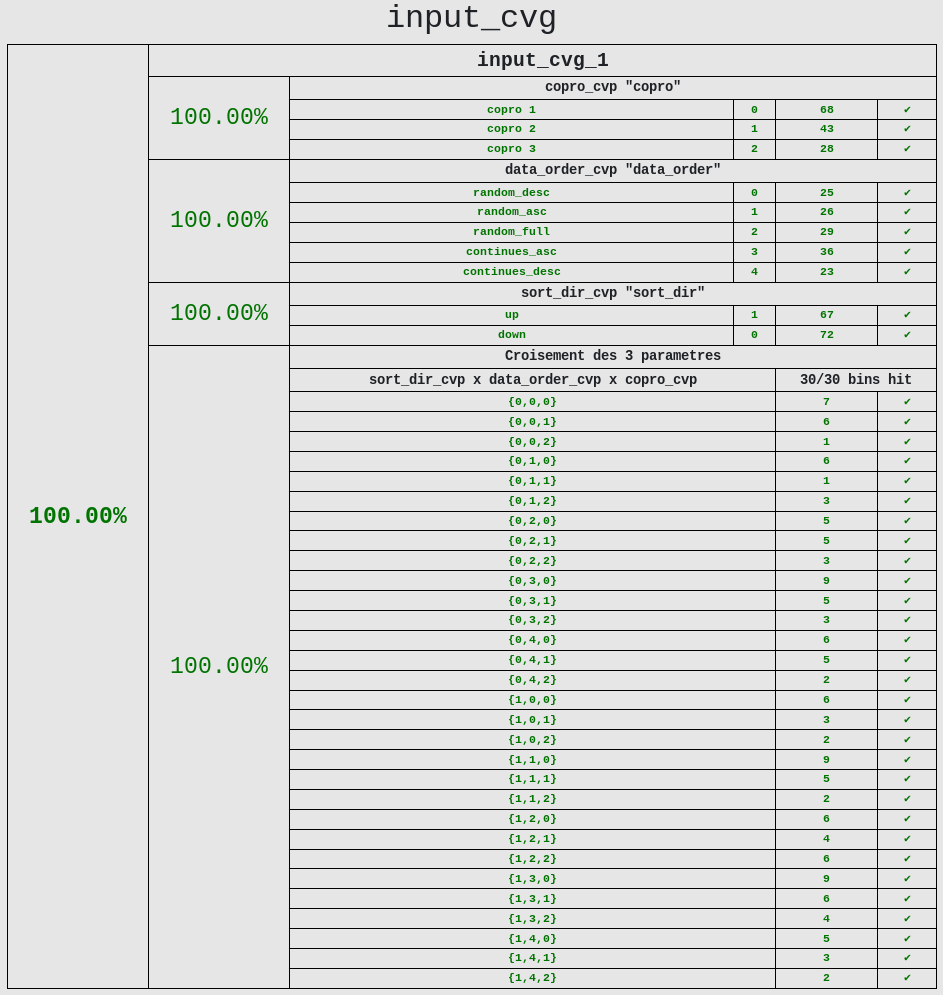
\includegraphics[width=\linewidth]{coverage}
	\caption{Résultats de FC4SC}
	\label{fig:fc4sc}
\end{figure}

\end{document}
